\documentclass[12pt]{amsart}
\usepackage[T1]{fontenc}
\usepackage[utf8]{inputenc}

\usepackage[top=1.95cm, bottom=1.95cm, left=2.35cm, right=2.35cm]{geometry}

\usepackage{hyperref}
\usepackage{enumitem}

\usepackage{stmaryrd}

\usepackage{tcolorbox}
\usepackage{multicol}
\usepackage{fancyvrb}
\usepackage{xstring}
\usepackage{amsmath}
\usepackage[french]{babel}
\usepackage[
    type={CC},
    modifier={by-nc-sa},
	version={4.0},
]{doclicense}
\usepackage{textcomp}
\usepackage{xcolor}
\usepackage{tcolorbox}

\usepackage{pgffor}
      
\usepackage{tnsmath}

    
\newtheorem{fact}{Fait}%[section]

\newtheorem{definition}{Définition}%[section]
\newtheorem{theorem}{Théorème}%[section]
\newtheorem{example}{Exemple}%[section]
\newtheorem{remark}{Remarque}%[section]
\newtheorem*{notations}{Notations}

\setlength\parindent{0pt}


\DeclareMathOperator{\taille}{\text{\normalfont\texttt{taille}}}

\newcommand\centerit[1]{%%
	\smallskip
	
	\begin{center}
		#1
	\end{center}
}


\newcommand\sheepnb[1]{mouton no.#1}

\newcommand\move[1]{\sheepnb{#1} va avancer}
\newcommand\lmove[1]{\move{#1} vers la gauche}
\newcommand\rmove[1]{\move{#1} vers la droite}

\newcommand\jump[1]{\sheepnb{#1} va sauter}
\newcommand\ljump[1]{\jump{#1} vers la gauche}
\newcommand\rjump[1]{\jump{#1} vers la droite}



% Source pour le \@tfor :
% 	* https://tex.stackexchange.com/a/253205/6880
\makeatletter
% Nothing special for the cell...	
	\newcommand\elasticbox[1]{%
		\fcolorbox{black}{white}{\normalfont #1}%
	}

	\newcommand\fixedboxcolored[3]{%
		\fcolorbox{#1}{#2}{\makebox[1em]{\normalfont #3}}%
	}

	\newcommand\fixedbox[1]{%
		\fixedboxcolored{black}{white}{\makebox[1em]{\normalfont #1}}%
	}

% ... will move
	\newcommand\elasticboxwill[1]{%
		\fcolorbox{black}{red!15}{\normalfont #1}%
	}

	\newcommand\fixedboxwill[1]{%
		\fixedboxcolored{black}{red!15}{\normalfont #1}%
	}

% ... has moved
	\newcommand\elasticboxhas[1]{%
		\fcolorbox{black}{black!10}{\normalfont #1}%
	}
	
	\newcommand\fixedboxhas[1]{%
		\fixedboxcolored{black}{black!10}{\normalfont #1}%
	}

% Let's go !
	\newcommand\@empty@content{\phantom{N}}
	\newcommand\emptycell{\fixedbox{\@empty@content}}
	\newcommand\white{\fixedbox{\bfseries B}}
	\newcommand\black{\fixedbox{\bfseries N}}
	
	\newcommand\@ellipsis@{\,\,\vphantom{N}$\cdots$\,\,}
	\newcommand\myellipsis{\elasticbox{\@ellipsis@}}

% ... will move
	\newcommand\emptycellwill{\fixedboxwill{\@empty@content}}
	\newcommand\whitewill{\fixedboxwill{\bfseries B}}
	\newcommand\blackwill{\fixedboxwill{\bfseries N}}
	\newcommand\myellipsiswill{\elasticboxwill{\@ellipsis@}}

% ... has moved
	\newcommand\emptycellhas{\fixedboxhas{\@empty@content}}
	\newcommand\whitehas{\fixedboxhas{\bfseries B}}
	\newcommand\blackhas{\fixedboxhas{\bfseries N}}
	\newcommand\myellipsishas{\elasticboxhas{\@ellipsis@}}

	\newcommand\config[1]{%
		\texttt{%
			\upshape%
			\@tfor\next:=#1\do{%
				\if\next .\kern.15em{\tiny\textbullet}\kern.15em\else%
					\next{}%
				\fi%
			}%
		}%
	}

% B : blanc normal
% N : noir normal
% . : vide normal
% - : ellipsis
%
% b : blanc qui va bouger
% n : noir qui va bouger
% v : vide qui va bouger
% = : ellipsis qui va bouger
%
% p : blanc qui vient de bouger
% u : noir qui vient de bouger
% a : vide qui vient de bouger
% + : ellipsis
%
% < Ouvre un cadre de surlignement de plusieurs cellules
% < Ferme un cadre de surlignement de plusieurs cellules
	\newcommand\gameline[1]{%
		\@tfor\next:=#1\do{%
			\if\next B\white{}\else%
		    \if\next N\black{}\else%
			\if\next .\emptycell{}\else%
			\if\next -\myellipsis{}\else%
			%
			\if\next b\whitewill{}\else%
		    \if\next n\blackwill{}\else%
		    \if\next v\emptycellwill{}\else%
			\if\next =\myellipsiswill{}\else%
		    %
			\if\next p\whitehas{}\else%
		    \if\next u\blackhas{}\else%
		    \if\next a\emptycellhas{}\else%
			\if\next +\myellipsishas{}\else%
		    %
\quad {\bfseries [[ illegal character : \, {\normalfont \next{}} \, ]]} \quad % BUG
			\fi%  :
			\fi%  a
			\fi%  u
			\fi%  p
			%
			\fi%  =
			\fi%  v
			\fi%  n
			\fi%  b
			%
			\fi%  -
			\fi%  .
			\fi%  N
			\fi%  B
		}%
	}
	

	\newcommand\autobox[1]{%
      \foreach \i in {1, ..., #1} {%
        \fixedbox{\i}%
      }
	}
	

	\newcommand\gamelineplus{\@ifstar{\@gamelineplus@star@}{\@gamelineplus@no@star@}}

	\newcommand\@gamelineplus@no@star@[2]{
		\gameline{#1}
		\setbox0=\hbox{#2\unskip}\ifdim\wd0=0pt \else {\small \ $\leftarrow$ #2}\fi
	}

	\newcommand\@gamelineplus@star@[2]{
		\@gamelineplus@no@star@{#1}{#2}
		
		\StrLen{#1}[\@length@]
		\noindent  
		\autobox{\@length@}
	}

	\newcommand\listbox[1]{%
		\@tfor\next:=#1\do{\fixedbox{\next}}%
	}
	
	
	\newcommand\iterconfig[1]{
		\foreach \k/\p in {#1}{
			\subsection{Configuration \texttt{\k N\kern.15em{\tiny\textbullet}\kern.15em\p B}}   
		 	\input{black-and-white-leapfrog/\k N\p B}
		}
	}
\makeatother


\newcommand\step[1]{\textbf{\texttt{[E#1]}}}

\newenvironment{mvts}[1][start=1]{
	\normalfont
	\begin{enumerate}[#1, left = 0pt .. 3em, label = \step{\arabic*}]
}{
	\end{enumerate}
}

\newcommand\factwin[2]{
	\begin{fact}
	La configuration \config{#1N.#2B} est résoluble.
	\end{fact}
}

 
\begin{document}

\title{BROUILLON - Un saute-mouton bicolore pour gloutons}
\author{Christophe BAL}
\date{13 Mars 2019}

\maketitle

\begin{center}
	\itshape
	Document, avec son source \LaTeX, disponible sur la page
	
	\url{https://github.com/bc-writing/drafts}.
\end{center}


\bigskip


\begin{center}
	\hrule\vspace{.3em}
	{
		\fontsize{1.35em}{1em}\selectfont
		\textbf{Mentions \og légales \fg}
	}
			
	\vspace{0.45em}
	\doclicenseThis
	\hrule
\end{center}

	
\bigskip
\setcounter{tocdepth}{2}
\tableofcontents


% ----------------- %


\section{Une devinette qui défrise}

Notre billard est un peu bizarre car il est juste constitué de deux demi-droites de même origine, et notre bille est dans le secteur angulaire le "plus petit" formé par ces deux bandes. Ceci se représente comme suit.

\medskip

\begin{center}
	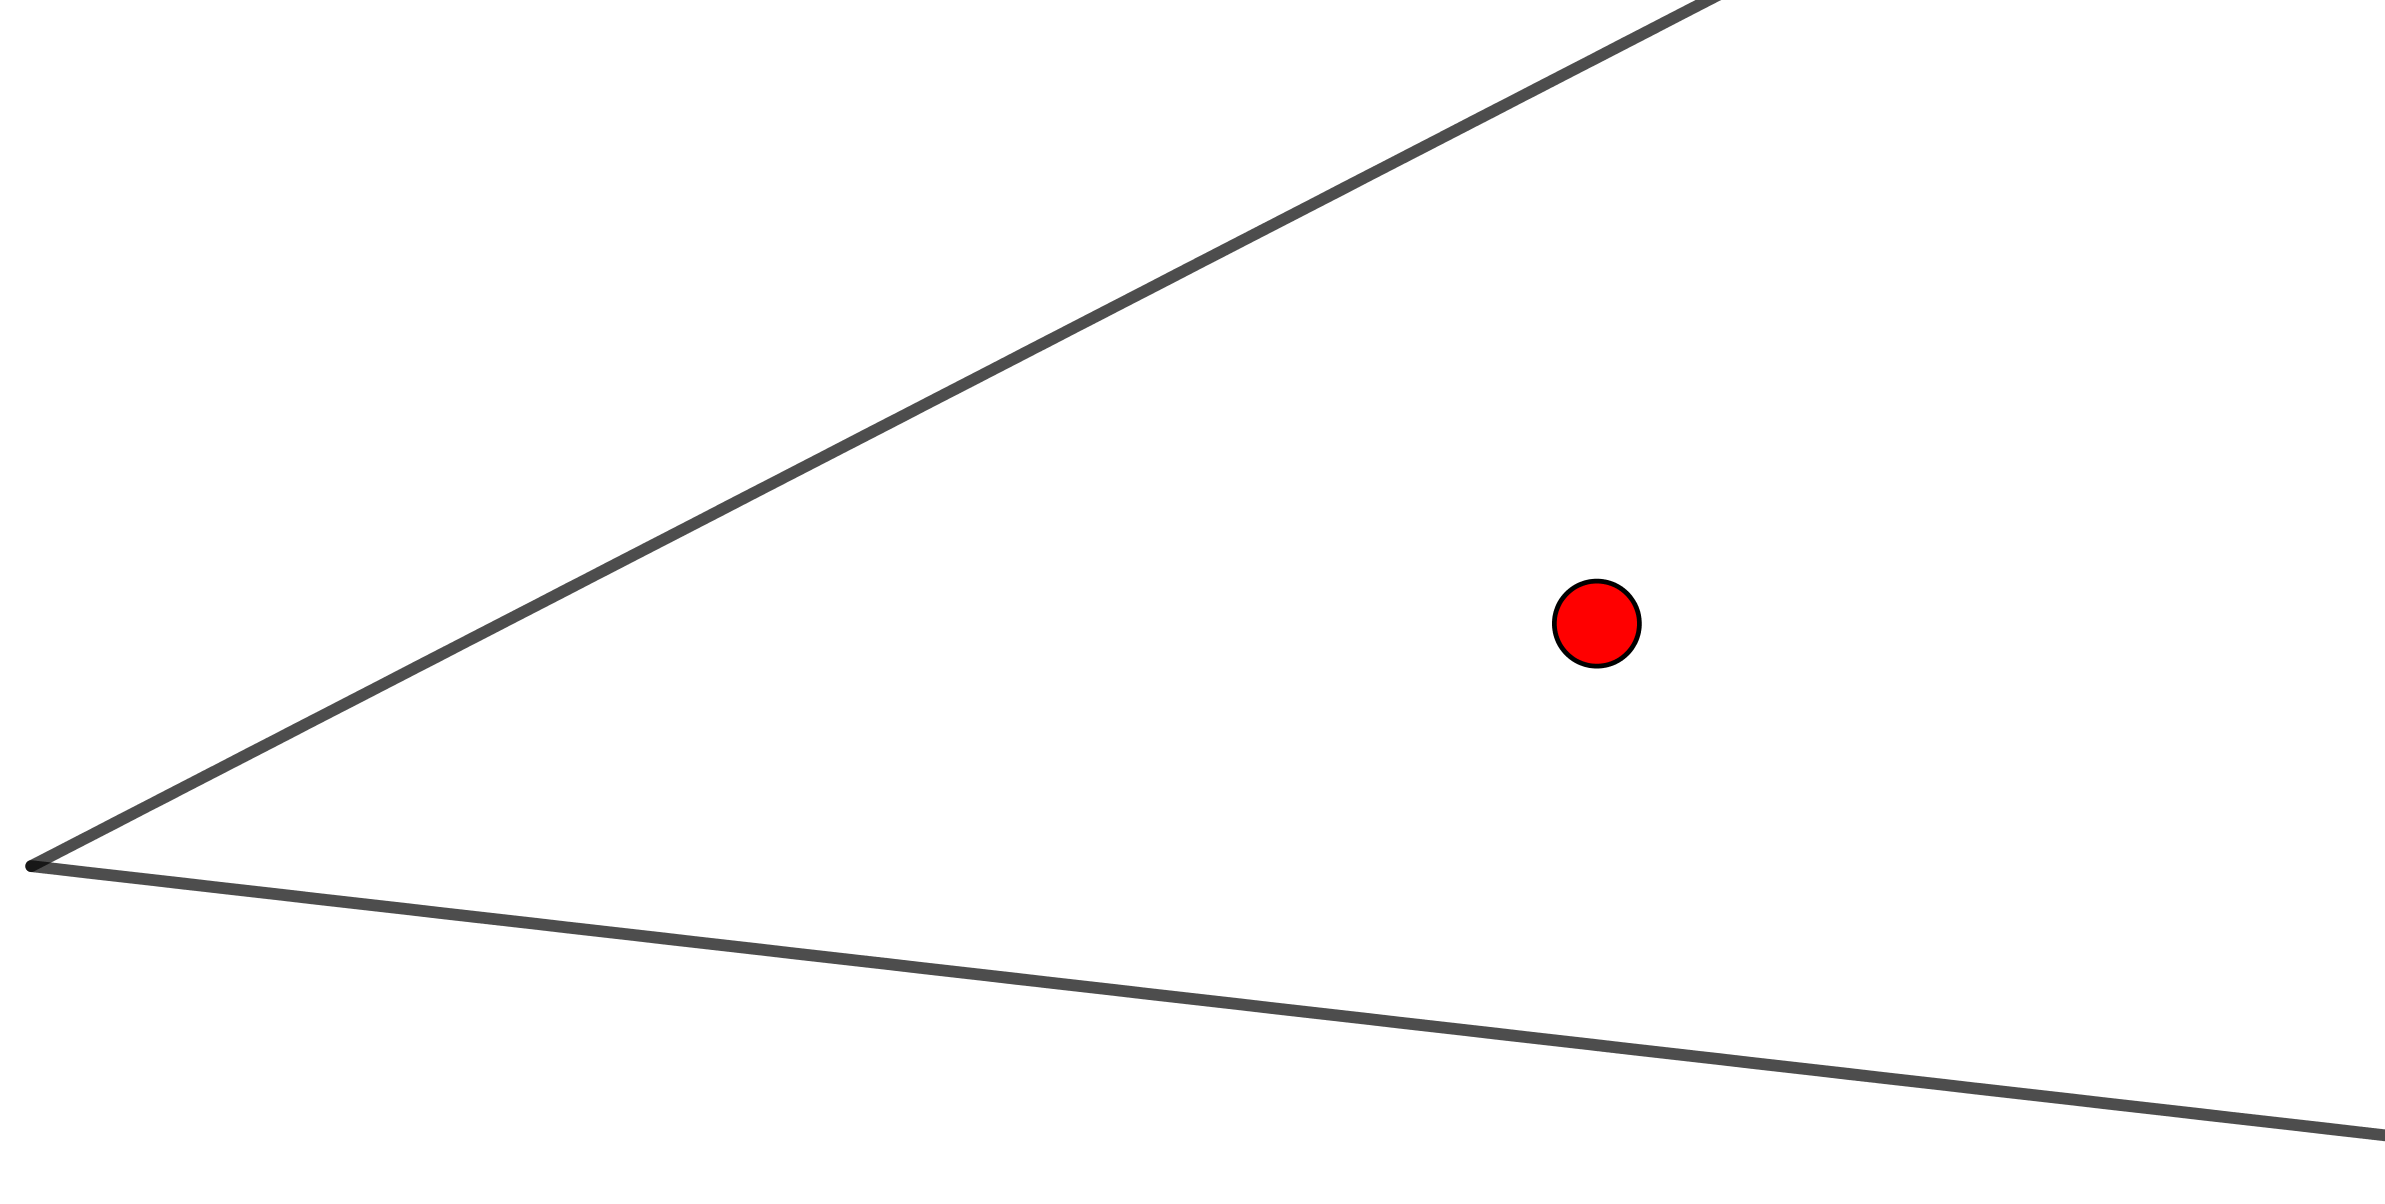
\includegraphics[width=12cm]{basic-math-pool/empty.png}
\end{center}

Dans la suite, nous considérons que notre bille est en fait un point, et du coup nous ne considérons pas les effets de rotation de la bille, et de plus nous ignorons les frottements, autorisant ainsi la bille à se balader vers l'infini et au-delà \emph{(tout ceci pour plus de réalisme)}.

\medskip

Concrètement, on pourrait se munir de deux miroirs plans verticaux et d'une source pouvant envoyer, dans un plan horizontal, un rayon laser dans une direction donnée.


% ----------------- %


\section{Vocabulaire et notations}

Dans la suite, nous utiliserons les notations suivantes.
\begin{itemize}
	\item $2\,\NN$ désigne l'ensemble des nombres naturels pairs.
	
	\item $2\,\NN + 1$ désigne l'ensemble des nombres naturels impairs.
	
	\item $\forall (n , m) \in \NN^2$, $n \vee m$ désigne le PPCM de $n$ et $m$.

	\item $\forall (n , m) \in \NN^2$, $n \wedge m$ désigne le PGCD de $n$ et $m$.

	\item $a \strictdivides b$ signifie que $a \divides b$ et $a \neq b$ (division stricte).

	\item $\PP$ désigne l'ensemble des nombres premiers.
	
	\item $\forall (p ; n) \in \PP \times \NNs$\,, $\padicval{n} \in \NN$ est la valuation $p$-adique de $n$\,, c'est-à-dire $p^{\padicval{n}} \divides n$\,, mais $p^{\padicval{n} + 1} \ndivides n$\,.
\end{itemize}


% ----------------- %


\section{Quelques configurations particulières}

Afin de nous construire une petite intuition pour la résolution, ou non, de la devinette des moutons, nous allons étudier quelques configurations simples.

\iterconfig{1/1, 2/1, 2/2, 3/2, k/1}


% ----------------- %


\section{Deux principes de symétrie}

Imaginons que nous soyons de part et d'autre de la ligne de jeux.
Pour vous les règles de déplacement et les couleurs sont inversés par rapport à moi.
Si je résous une configuration, vous pourrez aussi la faire avec la votre un peu particulière.
Ceci nous donne l'idée de chercher des principes de symétrie. Les faits suivants en proposent deux.



\begin{fact} \label{symmetry-color}
	La configuration \config{kN.pB} est résoluble si et seulement si la configuration \config{pN.kB} l'est aussi. 
	Par exemple, nous avons :
	
	\centerit{%
		\gameline{NNNN.BB} est résoluble.
		\, $\Longleftrightarrow$ \, 
		\gameline{NN.BBBB} est résoluble.
	}
	
	\medskip
	
	Plus généralement, considérons deux configurations $\setproba*{C}{1}$ et $\setproba*{C}{2}$ , et pour chaque $k \in \setgene{1 ; 2}$ notons $\setproba*{R}{k}$ la configuration obtenue en faisant un demi-tour et en échangeant les couleurs.
	Alors il existe des mouvements permettant de passer de $\setproba*{C}{1}$ à $\setproba*{C}{2}$ si et seulement si il en existe pour aller de $\setproba*{R}{1}$ à $\setproba*{R}{2}$ \emph{(attention à l'ordre des indices)}.  
\end{fact}


\begin{proof}
	Donnons un exemple d'application des transformations.
	\begin{enumerate}
		\item On applique un demi-tour à la ligne de jeu :
		\centerit{%
			\gameline{nnnn.pp}
			\, devient \, 
			\gameline{pp.nnnn} .
		}
		
		\noindent
		Tout mouvement ou saut fait dans un sens sur une ligne de jeu sera fait dans l'autre sens sur l'autre.

		\item Après le demi-tour, on échange les couleurs pour revenir aux règles classiques du jeu :
		\centerit{%
			\gameline{pp.nnnn}
			\, devient \,
			\gameline{uu.bbbb} .
		}
	\end{enumerate}
	
	Revenons au cas général.
	Si l'on peut passer de $\setproba*{C}{1}$ à $\setproba*{C}{2}$ alors il suffit de reprendre la même séquence de mouvements en échangeant les couleurs et les sens de parcours pour aller de $\setproba*{R}{1}$ à $\setproba*{R}{2}$ .
	Ceci s'applique en particulier à la résolution d'un jeu telle que nous l'avons indiquée. 
	Ceci est un petit truc tout bête qui va nous rendre un énorme service très bientôt.
\end{proof}


Redonnons les mouvements proposés pour résoudre la configuration \config{2N.2B}.
\begin{mvts}
	\medskip
	\item  \gameline{NN.bB}
	
	\medskip
	\item  \gameline{Nnp.B}
	
	\medskip
	\item  \gameline{n.BuB}
	
	\medskip
	\item  \gameline{.ubNB}
	
	\medskip
	\item  \gameline{pN.Nb}
	
	\medskip
	\item  \gameline{BNpn.}
	
	\medskip
	\item  \gameline{BnB.u}
	
	\medskip
	\item  \gameline{B.buN}
	
	\medskip
	\item  \gameline{Bp.NN}
\end{mvts}


Constatez-vous quelque chose ? Si vous regardez de part et d'autre de l'étape \step{5}, nous avons une autre forme de symétrie. Mettons-là en valeur.
\begin{multicols}{2}
	\medskip \step{1} 
	\gameline{nn.pp} \,\,\,\,\rotatebox[origin=c]{270}{$\Rsh$}
	
	\medskip \step{2} 
	\gameline{nnb.p} \quad $\shortdownarrow$
	
	\medskip \step{3} 
	\gameline{n.pup} \quad $\shortdownarrow$
	
	\medskip \step{4} 
	\gameline{.upup} \quad $\shortdownarrow$

	% ----------- %
	
	\medskip \hfill{} $\Rsh$ \quad \step{9}
	\gameline{pp.nn}

	\medskip \hfill{} $\shortuparrow$ \quad \step{8}
	\gameline{p.bnn}

	\medskip \hfill{} $\shortuparrow$ \quad \step{7}
	\gameline{pup.n}

	\medskip \hfill{} $\shortuparrow$ \quad \step{6}
	\gameline{pupu.}
\end{multicols}
\vspace{-1em}
\begin{center}
	\medskip \rotatebox[origin=c]{180}{$\Lsh$} \, $\shortrightarrow$ \quad \step{5}
	\gameline{BN.NB} \quad $\shortrightarrow$ \, \rotatebox[origin=c]{270}{$\Lsh$}
\end{center}

Ceci motive le fait général suivant.


\begin{fact} \label{symmetry-no-color}
	Considérons deux configurations $\setproba*{C}{1}$ et $\setproba*{C}{2}$ , et pour chaque $k \in \setgene{1 ; 2}$ notons $\setproba*{R}{k}$ la configuration obtenue en faisant juste un demi-tour sans échanger les couleurs.
	Alors il existe des mouvements permettant de passer de $\setproba*{C}{1}$ à $\setproba*{C}{2}$ si et seulement si il en existe pour aller de $\setproba*{R}{2}$ à $\setproba*{R}{1}$ \emph{(attention à l'ordre des indices)}.
\end{fact}


\begin{proof}
	Il suffit de raisonner sur deux étapes successives en considérant les différents mouvements possibles.
\end{proof}



% ----------------- %


\section{Résolution de la configuration \texttt{kN$\cdot$kB}}

Les démonstrations ci-dessous sont sans astuce particulière et faites en raisonnant sur la ligne de jeu telle que nous la connaissons. Autrement dit, nous n'allons pas travailler avec une représentation ad-hoc du jeu.


\begin{remark}
	Dans la suite, pour ne pas alourdir le document, nous indiquerons d'un seul coup plusieurs mouvements successifs.
	Par exemple, voici une méthode possible pour résoudre la configuration \config{3N.3B} qui va au passage nous éclairer pour le cas général.
	\begin{mvts}
		\medskip
		\item  \gamelineplus{NNN.bBB}{Un seul blanc peut bouger.}

		\medskip
		\item  \gamelineplus{Nnnp.BB}{Deux noirs peuvent bouger.}

		\medskip
		\item  \gamelineplus{N.ububb}{Trois blancs peuvent bouger.}

		\medskip
		\item  \gamelineplus{npnpnp.}{Trois noirs peuvent bouger.}

		\medskip
		\item  \gamelineplus{.bububu}{Par symétrie, on sait que l'on va gagner. Voir le fait \ref{symmetry-no-color}.}
	\end{mvts}

	Notons au passage la configuration particulière de l'étape \step{4} car ceci va être important pour notre preuve du cas général. 
\end{remark}



\begin{fact} \label{kNkB-reduction}
	Soit $k \in \NNs$. Suivant la parité de $k$ nous avons :
	\begin{enumerate}
		\item Si $k = 2r$ est pair, nous pouvons passer de \config{kN.kB} à \config{kNB.} .

		\item Si $k = 2r+1$ est impair, nous pouvons passer de \config{kN.kB} à \config{.kNB} .
	\end{enumerate}
\end{fact}


\begin{proof}
	Ceci découle du résultat plus général suivant en prenant $m = 0$.
\end{proof}



\begin{fact}
	Soit $(k ; m) \in \NN^2$. Suivant la parité de $k$ nous avons :
	\begin{enumerate}
		\item Si $k = 2r$ est pair, nous pouvons passer de \config{kNmNB.kB} à \config{(k+m)NB.} .

		\item Si $k = 2r+1$ est impair, nous pouvons passer de \config{kNmNB.kB} à \config{.(k+m)NB} .
	\end{enumerate}
\end{fact}


\begin{proof}
	Pour $j \in \NN$, notons $\setproba*{P}{j}$ la propriété \emph{\og $\forall m \in \NN$, $\forall k \in \NN$ tel que $0 \leq k \leq j$ , soit (1) est vrai, soit (2) est vrai \fg}.
	Prouvons $\setproba*{P}{j}$ par récurrence sur $j \in \NN$.
	
	\begin{itemize}[label=\small\textbullet]
		\item \textbf{Cas de base :} pour la suite nous devons à la fois prouver $\setproba*{P}{0}$ et $\setproba*{P}{1}$ .
		
		\noindent
		$\setproba*{P}{0}$ est clairement vérifiée puisque $\setproba*{P}{0}$ est \emph{\og $\forall m \in \NN$, nous pouvons passer de \config{mNB.} à \config{(0+m)NB.} \fg} .
		
		\noindent
		Passons à $\setproba*{P}{1}$ . Nous devons valider la proposition \emph{\og $\forall m \in \NN$, nous pouvons passer de \config{1NmNB.1B} à \config{.(1+m)NB} \fg} .
		Les cas $m = 0$ et $m = 1$ sont faciles à traiter, tandis que pour $m \geq 2$ , il suffit de faire les mouvements suivants.
	\begin{mvts}
		\medskip
		\item \gamelineplus{nnB-nB.B}{Du type \config{1NmNB.1B} .}

		\medskip
		\item \gamelineplus{.uB-uBuB}{Du type \config{.(1+m)NB} .}
	\end{mvts}


		\item \textbf{Hérédité :} supposons que $\setproba*{P}{j}$ avec en plus $j \geq 1$. On peut faire ceci car si $j = 0$ alors $j + 1 = 1$ donne un cas qui a déjà été traité. Nous devons alors déduire $\setproba*{P}{j+1}$ de $\setproba*{P}{j}$.
		
		\medskip
		
		\noindent
		Si $m = 0$ alors nous faisons les mouvements suivants.
		\begin{mvts}
			\medskip
			\item \gamelineplus{-NNn.BBB-}{Du type \config{(j+1)N0NB.(j+1)B} .}

			\medskip
			\item \gameline{-NN.ubbB-}

			\medskip
			\item \gamelineplus{-NNpNp.B-}{Du type \config{(j-1)N2NB.(j-1)B} .}
		\end{mvts}
			
		\noindent
		Comme $j - 1 \geq 0$ et $j + 1 \geq 2$ sont de même parité, la validité de $\setproba*{P}{j}$ permet, si $j+1 = 2r+1$ est impair, d'arriver à \config{.(j-1+2)NB} c'est à dire à \config{.(j+1)NB} , et sinon d'arriver à \config{(j+1)NB.} .
			
		\medskip
			
		\noindent
		Si $m \geq 1$ alors nous faisons les mouvements suivants avec un abus de notations évidents pour les \, \gameline{NB} \, centraux si $m = 1$ mais ceci n'invalide pas le raisonnement fait.
		\begin{mvts}
			\medskip
			\item \gameline{-NNnnB-nB.BBB-}

			\medskip
			\item \gameline{-NN.ub-ububbB-}

			\medskip
			\item \gameline{-NNpNp-NpNp.B-}
		\end{mvts}
			
		\noindent
		La dernière configuration étant du type \config{(j-1)N(m+2)NB.(j-1)B} , nous pouvons de nouveau arriver à \config{.(j+1+m)NB} ou \config{(j+1+m)NB.} suivant la parité de $(j+1)$.
	\end{itemize}
\end{proof}


 
\begin{fact} \label{kNkB-resoluble}
	$\forall k \in \NNs$, la configuration \config{kN.kB} est résoluble.
\end{fact}


\begin{proof}
	Distinguons deux cas avec des abus de notations évidents qui sont juste là pour faciliter la compréhension.

	\begin{itemize}[label=\small\textbullet]
		\item  Supposons que $k = 2r$ soit pair. Nous pouvons alors faire les mouvements suivants d'après le fait \ref{kNkB-reduction}.
		\begin{mvts}
			\medskip
			\item \gameline{-NNN.BBB-}

			\medskip
			\item \gameline{nBnB-nB.}

			\medskip
			\item \gameline{.Bu-BuBu}
		\end{mvts}
		
		\noindent
		Comme les configurations des étapes \step{2} et \step{3} sont symétriques, en reprenant les mouvements à rebours de \step{2} à \step{1} et en échangeant juste les sens de parcours, et non les couleurs, nous arrivons finalement à la configuration symétrique de  \, \gameline{-NN.BB-} \, qui est \, \gameline{-BB.NN-} \, ce qui nous fait gagner \emph{(voir le fait \ref{symmetry-no-color})}.


		\item Supposons que $k = 2r + 1$ soit impair. Nous pouvons alors faire les mouvements suivants de nouveau en faisant appel au fait \ref{kNkB-reduction}.
		\begin{mvts}
			\medskip
			\item \gameline{-NNN.BBB-}

			\medskip
			\item \gameline{.NbNb-Nb}

			\medskip
			\item \gameline{pN-pNpN.}
		\end{mvts}
		
		\noindent
		Nous pouvons conclure comme précédemment avec un argument de symétrie.
	\end{itemize}
\end{proof}



\begin{remark}
	Si vous reprenez les preuves de cette section, vous noterez que nous avons de nouveau appliquer une tactique gloutonne en commençant par faire bouger un mouton noir. \textbf{Nous avons une preuve algorithmique constructive !}
\end{remark}





% ----------------- %


\section{Résolution de la configuration \texttt{kN$\cdot$pB}}

\input{black-and-white-leapfrog/kNpB-proof}







\bigskip

\hrule

\section{AFFAIRE À SUIVRE...}

\bigskip

\hrule


% ----------------- %

%
%\section{Un algorithme à utiliser et étudier}
%
%\input{black-and-white-leapfrog/algorithm}
%

%% ----------------- %
%
%
%\section{Une preuve astucieuse ?}
%
%\input{black-and-white-leapfrog/trickyproof}
%
%
%% ----------------- %
%
%
%\section{Unicité ?}
%
%\input{black-and-white-leapfrog/uniqueness}

\end{document}
